\chapter{研究方法}

本研究將 Bare-Metal Provisioning 區分成以下四個部分:

\begin{enumerate}
\item 遠端控制
\item 裸機再生
\item 映像檔部署
\item 系統組態設定
\end{enumerate}

\section{遠端控制}
由於本研究的目標主機群是一般個人電腦,並不具備有伺服器管理功能的 IPMI ,因此 BitFission 將透過 Wake-On-Lan、PXE 和 Ansible,進行 Bare-Metal 遠端控制與組態設定。即使沒有 IPMI 遠端管理功能,BitFission 仍可以完成目標主機群的電源控制、自動化部署與組態設定。


\section{裸機再生}
\subsection{BitAtom}
\begin{figure}[!htbp]
\centering
\scalebox{.5}{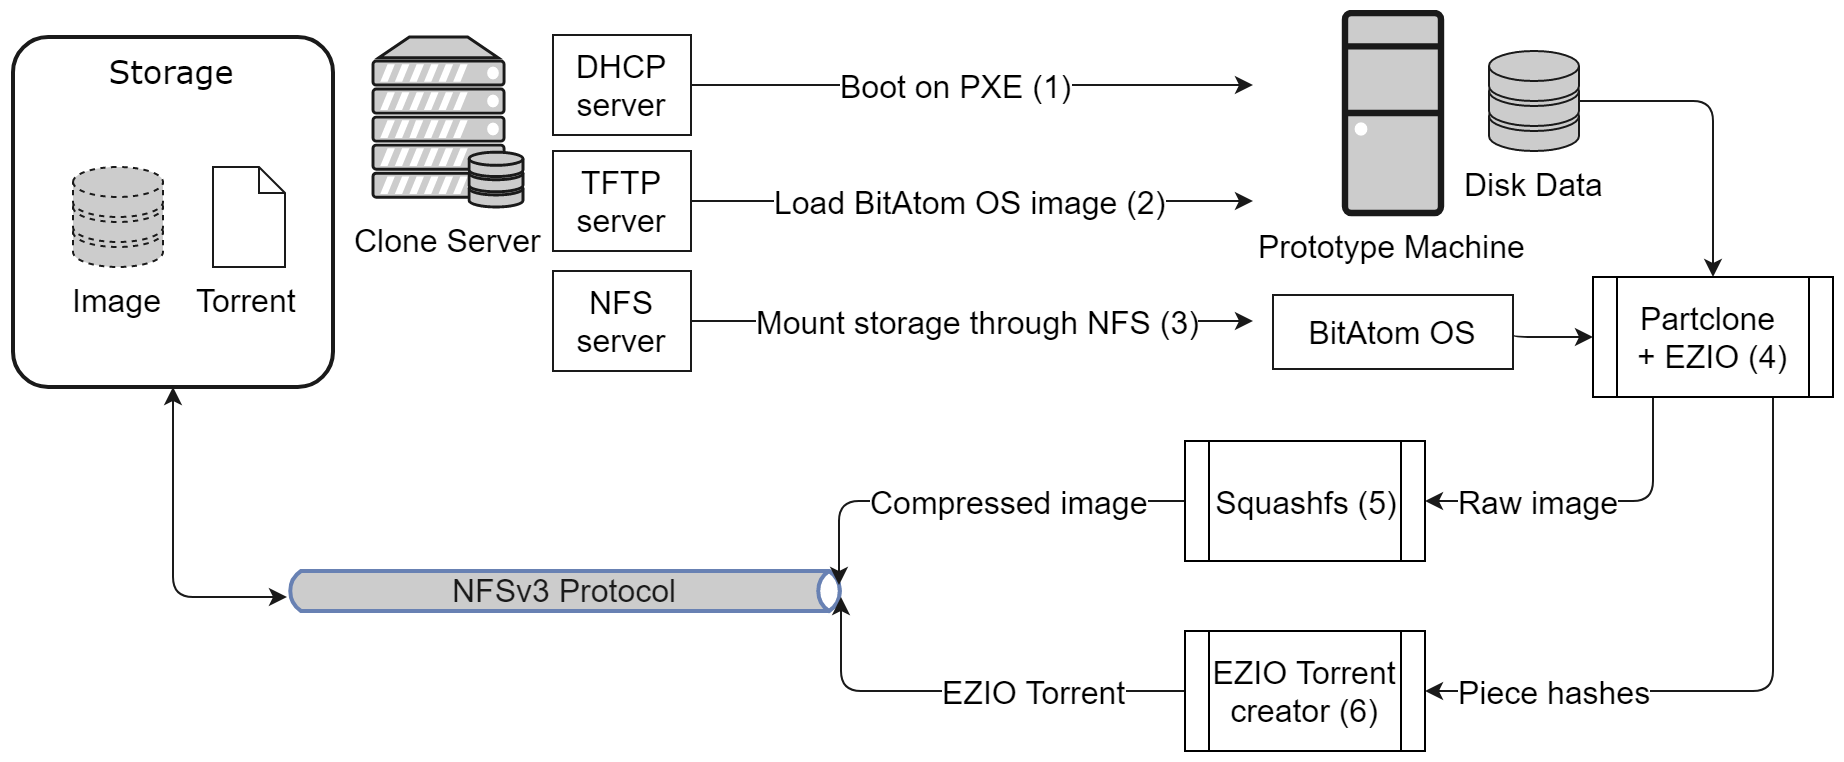
\includegraphics{images/BitAtom_Flowchart.png}}
\caption{BitAtom Flowchart.}
\label{i:bitatomflowchart}
\end{figure}


為了自動化產生映像檔,本研究使用 archiso 客製化了自動備份的特務作業系統 BitAtom,BitAtom 包含 Partclone、NFS client 以及自動化再生映像檔的腳本。
裸機再生流程如圖 \ref{i:bitatomflowchart}。
完整的再生伺服器包含了三項服務(services):DHCP 伺服器、TFTP 伺服器和 NFS 伺服器。
由於原型機本身是電腦教室中的個人電腦,開機時會優先從 PXE 開機,我們將 DHCP 伺服器中的 next-server 指向再生伺服器的 TFTP 伺服器(1),使原型機開機後從 TFTP 上下載 bootloader,再經由 bootloader 載入 TFTP 上的 BitAtom 映像檔(2)。BitAtom 作業系統會依據 TFTP 伺服器上的設定檔或是人工設定進行部署作業,有四項主要設定(參考原始碼 \ref{bitatom}):
\begin{enumerate}
\item NFS 伺服器 IP 位置
\item NFS 路徑
\item 映像檔儲存路徑
\item 目標再生硬碟
\end{enumerate}
BitAtom 會依照上述設定將指定的 NFS 掛載起來(3),並開始執行 Partclone 進行裸機再生,將硬碟資料拷貝至映像檔中(4)。
映像檔會透過 SqaushFS 進行壓縮(5)後在儲存至 NFS 上。
此外,製作映像檔產生的片段雜湊值將會透過程式轉換成種子檔(6)。
這樣一來就具備部署用的映像檔與種子檔了。

\subsection{Partclone}
Partclone 是一個製作分割區映像檔的工具程式,能夠分析檔案系統中的 bitmap,只把分割區中有使用的區塊寫入映像檔中,有效降低映像檔的大小,並且在還原的時候,因為需要讀取跟寫入的資料量減少,提高還原速度。Partclone 支援絕大多數的檔案系統,如 ext2、ext3、ext4、reiserfs、reiser4、xfs、jfs、btrfs、FAT12、FAT16、FAT32、NTFS、HFS、UFS。EZIO 原本也是使用 Partclone 製作映像檔,但是 EZIO 為了支援一般的 BitTorrent 軟體,修改了 Partclone 將每個區塊寫入不同的檔案,產生了許多零碎小檔案且無法進行 pipe 和壓縮功能,與 Partclone 原生的映像檔相比,占用的硬碟空間超過兩倍以上。
因此本研究決定沿用 Partclone 原生映像檔格式,並且自行開發 BitTorrent 部署軟體解讀 Partclone 原生的映像檔格式,這樣我們便能透過 pipe 與壓縮,使映像檔的保存更加方便有效率。


\subsection{整合 EZIO 與 Partcone} \label{ezio_and_partclone}
\begin{figure}[!htbp]
\centering
\scalebox{.4}{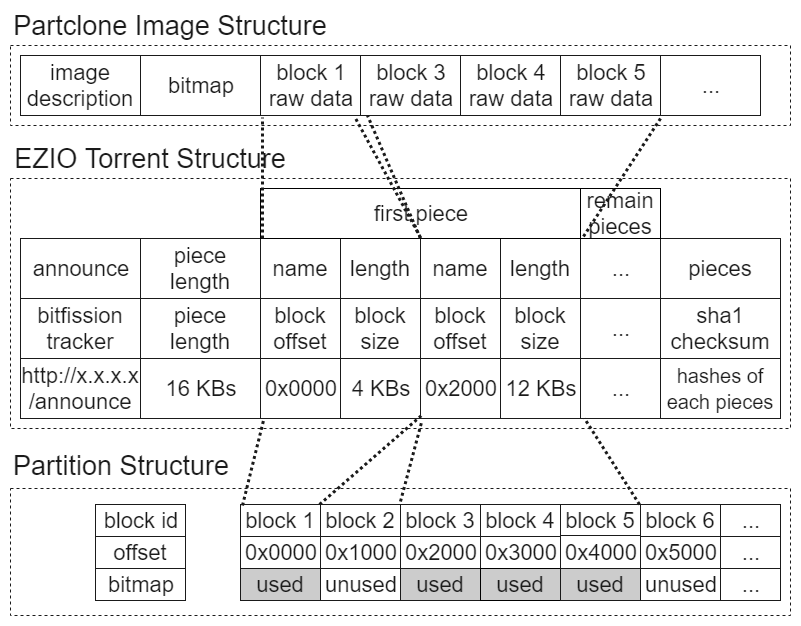
\includegraphics{images/torrent_partition_mapping.png}}
\caption{Torrent Structure.}
\label{i:torrent}
\end{figure}

EZIO 為了能夠把映像檔中每一個區塊正確寫入硬碟上相對應的 offset,我們需要有一個對映映像檔與硬碟分割區的種子檔(torrent) ,同時這個種子檔必須要符合 BitTorrent 協議,才能讓 EZIO 正確解讀。
因此 EZIO 在種子檔上建立了對映表的資訊,如圖\ref{i:torrent}所示,EZIO 將區塊的 offset 作為檔案名稱,以區塊的大小作為檔案長度,並且將連續的區塊合併當作一個檔案提高種子檔的資訊密集度。


為了要產生上述格式的種子檔 ,本研究在 Partclone 備份(Clone)過程中插入製作種子檔的程式碼,當 Partclone 每一次讀取 區塊 的過程中連帶計算種子檔所需要的雜湊值(pieces checksum) 、區塊 offset 和 區塊大小,如此方法不僅能夠產生種子檔同時也能省去重新讀取硬碟資料的時間。


\subsection{SquashFS}
%*TODO 用 Squashfs 和 zstd 進一步解決大型映像檔問題並且能夠些微提高傳輸效率*
%*bash 指令*
Partclone 製作的區塊層級映像檔往往會占用大量的儲存空間,因此 Clonezilla S.E. 會透過 zlib 等壓縮演算法對映像檔進行壓縮,減少所需的儲存空間。
然而 BitTorrent 協議無法確保循序讀取映像檔,因此不能透過串流的方式解壓縮映像檔,必須要使用支援隨機讀取解壓縮程式。
最初本研究使用了 archivemount 進行測試,發現其在隨機讀取的狀況下效能低落,拖垮映像檔傳輸的速度。
轉而此用 SquashFS,SquashFS 可以使用不同的壓縮演算法,將來源資料轉換成一個唯讀壓縮檔案系統。
本研究透過串流的方式,直接將 Partclone 的輸出導入 mksquashfs,將映像檔轉換成 SquashFS 格式的壓縮檔,請參考原始碼 \ref{bitatom}第 31 行。
然而若使用 zlib 壓縮演算法,仍有可能影響傳輸速率,因此本研究參考了 Zstd 與其他演算法的比較(表 \ref{t:compressor}) ,選擇了 lz4 作為 SquashFS 的壓縮演算法,雖然壓縮比率較差,但極佳的解壓縮速率讓 BitTorrent 傳輸不受其限制。
\begin{table}[!htbp]
\centering
\caption{壓縮演算法比較\cite{zstdbenchmarks}}
\label{t:compressor}
\begin{adjustbox}{max width=0.92\textwidth}
\begin{tabular}{lrrrrrr}

\toprule
\multicolumn{1}{l}{\textbf{壓縮演算法}} & \textbf{壓縮比} & \textbf{壓縮速率} & \textbf{解壓縮速率} \\ \midrule
\multicolumn{1}{l}{\textbf{lz4 1.7.5}} & \textbf{2.101} & \textbf{720MB/s} & \textbf{3600MB/s} \\

\multicolumn{1}{l}{\textbf{zstd 1.1.3-1}} & \textbf{2.877} & \textbf{430MB/s} & \textbf{1110MB/s} \\

\multicolumn{1}{l}{\textbf{zlib 1.2.8-1}} & \textbf{2.743} & \textbf{110MB/s} & \textbf{400MB/s} \\

\multicolumn{1}{l}{\textbf{lzo1x 2.09-1}} & \textbf{2.108} & \textbf{650MB/s} & \textbf{830MB/s} \\

\multicolumn{1}{l}{\textbf{lzf 3.6-1}} & \textbf{2.077} & \textbf{400MB/s} & \textbf{860MB/s} \\

\bottomrule
\end{tabular}
\end{adjustbox}
\end{table}


\section{映像檔部署}
\subsection{BitFission 部署系統架構}

\begin{figure}[!htbp]
\centering
\scalebox{.24}{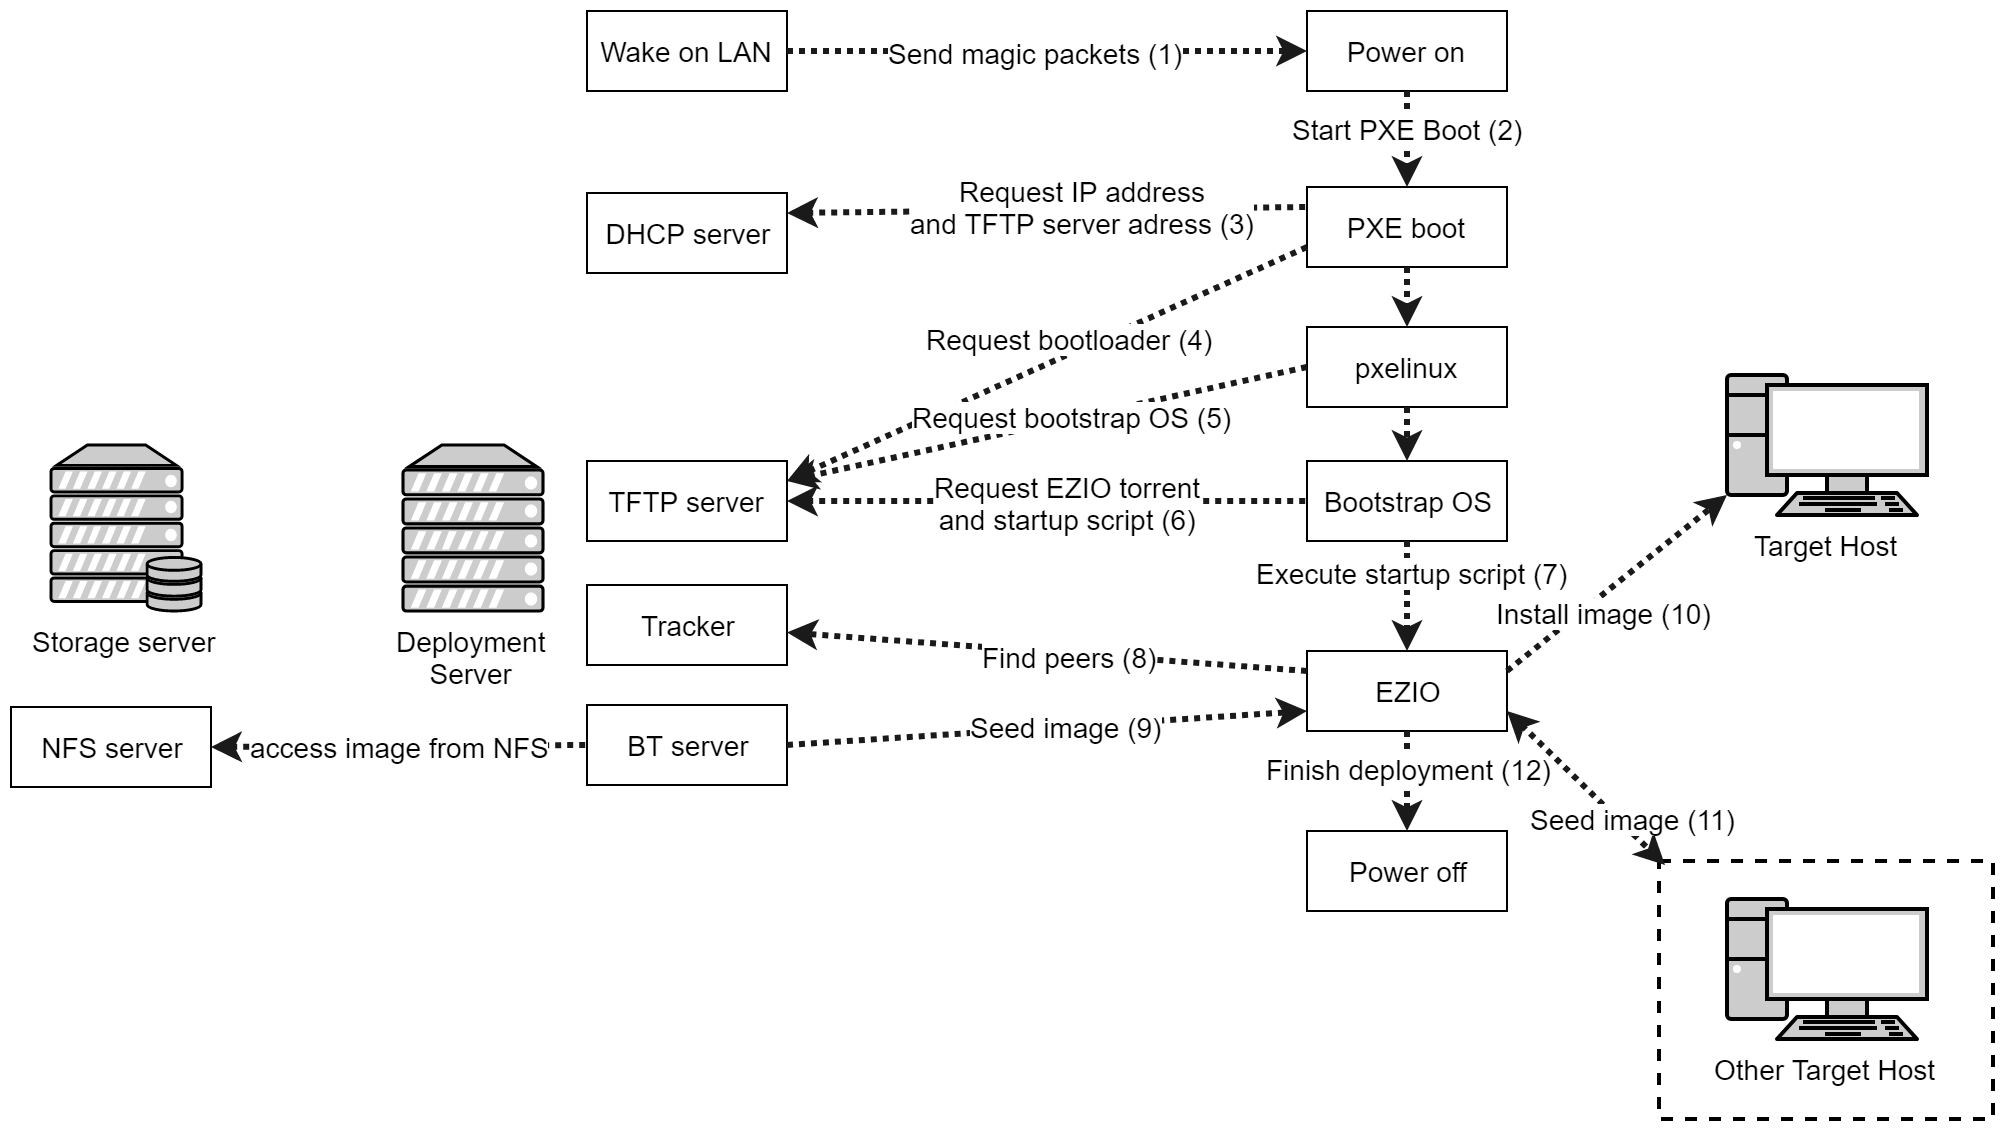
\includegraphics{images/BitFission_Deploy_Flowchart.png}}
\caption{BitFission Deployment Flowchart.}
\label{i:bitfissionflowchart}
\end{figure}


圖 \ref{i:bitfissionflowchart} 是 Bitfission 部署流程圖,我們透過 Wake-On-LAN 將目標主機喚醒(1),使其進入 PXE 開機模式(2),
自動向部署系統的 DHCP 伺服器請求 IP 與 TFTP 伺服器位置(3),
用以載入 Bootloader (4),Bitfission 使用 Pxelinux 作為 Bootloader 將部署用系統載入主機(5)。
部署用系統會自動向 TFTP 伺服器請求部署腳本與 EZIO 種子檔(6),
隨後透過部署腳本寫入磁碟分割表並啟動 EZIO 開始部署作業(7)。
EZIO 透過種子檔內容向 Tracker 發送請求,尋找可以提供映像檔的主機(8)。
此時 BitFission BT 伺服器便會與目標主機進行傳輸作業(9)。
EZIO 會直接將接收到的片段寫入硬碟區塊之中(10),並且透過 BitTorrent 協定分享給其他目標主機(11)。
傳輸完成後便會關機等待下一階段的部署作業。


%然而在部署之前,需要解決下述幾項議題。
%首先 EZIO 原先的映像檔是自製的規格無法兼容於 Partclone 原生的映像檔,因此 BitFission 的部署伺服器必須要當兩者之間的橋樑,本研究在部署程式中透過映像檔的 bitmap 將 piece 的 offset 轉換成映像檔的 offset 後,在從映像檔中讀取資料並且傳輸給 EZIO 的 BT 客戶端,如圖 \ref{i:flowchart} 所示,只要從映像檔讀取正確的 piece 並傳輸給 EZIO BitTorrent client 就可以還原硬碟資料。
%第二,BT 下載者與上傳者需要透過 tracker 傳遞資訊才能連結彼此,因此 BitFission 使用 Opentracker 架設 tracker 服務,並且可以利用 Opentracker 平均分布流量,避免下載者全部擠向同一個上傳者。第三,如何讓客戶端載入 ezio 系統

%\subsection{BitFission 部署伺服器}
%部署伺服器由哪些元件組成

\subsection{EZIO}
二〇一七年由臺灣國立交通大學研究生黃宇強和顏靖軒共同的開發基於 BitTorrent 協議的硬碟部署軟體 EZIO\cite{ezio},透過 libtorrent 函式庫實作了基於 BitTorrent 傳輸的硬碟部署方法。
由於 BitTorrent 協議的去中心化設計,透過 peer-to-peer 傳輸檔案有效利用每個主機節點的硬體資源,使得效率接近 Multicast ,在實際的應用下甚至勝過 Multicast 。
且 BitTorrent 協議具備非同步的特性,部署時不受單一主機異常而影響其他主機,異常主機也可以在一定時間內重新回到部署作業中。
而 EZIO 使用了當中最成熟的 libtorrent 函式庫作為 EZIO 的開發基底,效能比起其他 BitTorrent 函式庫更好。
綜合上述 EZIO 與 BitTorrent 的特性,本研究認為 EZIO 適合作為部署程式的載體,再由 BitFission 提供額外的輔助機制便能達成自動化部署。

\subsection{BT Server}
\begin{figure}[!htbp]
\centering
\scalebox{.56}{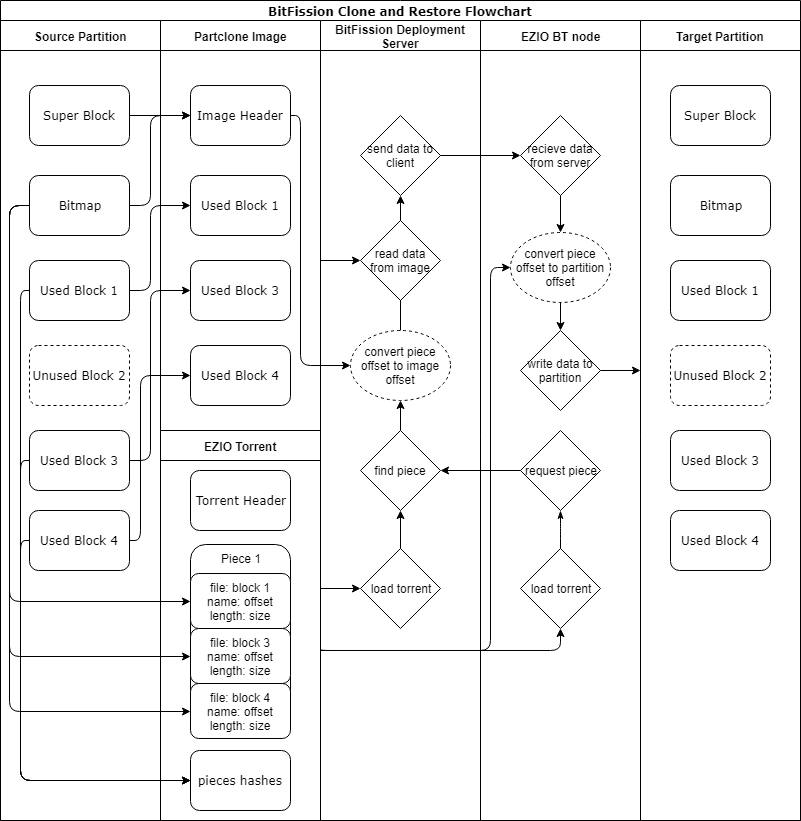
\includegraphics{images/BitFission_Clone_Flowchart.png}}
\caption{BitFission Flowchart.}
\label{i:flowchart}
\end{figure}

在圖 \ref{i:bitfissionflowchart} 中,BT Server 用以作為 BitTorrent 協議的播種伺服器(seeding server),是 BitFission 對等式網路部署的映像檔源頭。
由於要整合 EZIO 和 Partclone 的映像檔 [\ref{ezio_and_partclone}] ,我們不能使用無法解析 Partclone 映像檔格式的一般BitTorrent 軟體,因此本研究透過 libtorrent 函式庫自行撰寫了能夠讀取 Partclone 映像檔的 BitTorrent 軟體:BT Server。

圖 \ref{i:flowchart} 是 BT Server 與 EZIO 溝通的流程圖,BT Server 與 EZIO 皆載入由 Partclone 產生的 EZIO 種子檔,由 EZIO 發送片段請求給 BT Server,BT Server 解讀種子檔與 Partclone 映像檔後,回傳對應的片段至 EZIO,EZIO 在將之寫入硬碟之中。
原始碼 \ref{readv} 是 BT Server 中解讀 Partclone 映像檔格式的函式 readv,readv 是 libtorrent storage\_interface 中讀取來源檔案的函式,本研究透過 overwrite readv 函式來讀取映像檔。
在第21行可以看到如何計算 EZIO 片段與Partclone 映像檔區塊的對應。
首先映像檔本身包含標頭檔(header),我們需要偏移標頭檔大小,即 image\_head\_size。
再者是 libtorrent 讀取當前片段(piece)的偏移,即 offset。最後是先前片段的長度總和,即 piece*piece\_length()。
三者總和便是 libtorrent 讀取所需片段在 Partclone 映像檔上需要偏移的長度。
取得偏移長度後,第22至30行從偏移位置讀取映像檔資料並將該片段回傳,隨後 BT Server 將片段傳輸給 EZIO 客戶端。


%\subsection{BitTorrent Tuning}

\section{系統組態設定}
%依前面章節所述,如今組態管理工具已發展成熟,本研究採用既有的工具開發 BitFission 的組態管理系統。
%而組態管理的方式可分為推播式或拉取式,本研究在兩者中各取其一做比較,並以此決定使用哪種模式的工具。
組態管理系統是作業系統部署後,調整組態設定不可或缺的一部分。近年組態管理工具蓬勃發展,現已有許多成熟發展的開放原始碼專案可以進行軟體開通(software provisioning)、組態管理和應用程式部署(application deployment),如:
\begin{enumerate}
\item Ansible\cite{ansible}
\item Puppet\cite{puppet}
\end{enumerate}
本研究認為 Ansible 最適合作為 BitFission 後續設定的組態管理工具。
原因是由於 Ansible 的 agentless 架構,不必安裝額外的程式,以及其連線機制是透過 ssh 或 winrt ,可以自由的整合不同作業系統,包含 Unix-like 和 Windows 作業系統。
此外,Ansible 也不用在部署時在映像檔加入憑證,如 Puppet 是透過憑證認證,每台主機必須事先產生不同憑證才能夠與 Puppet master 進行組態設定。
最後還有 Ansible 是透過 push 的方式部署設定,相較於 Puppet 的 pull 機制,能夠即時回饋部署狀態便於 Provinioner 進行監控。
綜合以上優點,本研究決定採用 push 機制的 Ansible 作為 Bare-Metal 主機群的組態管理系統核心。映像檔部署後所需的部署後設定(post-deployment configuration),BitFission 利用 Ansible 調整每台主機的差異部分,例如修改主機名稱、網路設定、加入 Active Directory 和調整機碼(registry)等等部署後設定。

以交大資工系計中電腦教室為例,本研究編寫了 7 個 Ansible playbook,分別使用於:
\begin{enumerate}
\item 對應 IP 位置修改主機名稱
\item Windows 作業系統 KMS 認證
\item 一般軟體授權
\item 更新印表機資訊
\item 加入 Windows AD 網域
\item 更新 GPO 政策
\item 更變 SID 數值
\end{enumerate}
設定過程中即便需要重新啟動,也可透過 Ansible 自動化完成,部署人員僅需觀察 Ansible-playbook 執行結果,如有異常的主機,Ansible 亦提供 ad-hoc 讓部署人員直接對異常主機進行檢測。
